\chapter{Задание}

Разработать программное обеспечение, предоставляющее возможность генерации последовательностей случайных чисел алгоритмическим и табличным спобом, а также возможность расчета коэффициента критерия случайности по полученным последовательностям.

\chapter{Теоретическая часть}
\section{Получение последовательностей случайных чисел}
\subsection{Алгоритмический метод}

Для получения последовательности случайных чисел используется квадратичный конгруэнтный метод, который представим следующей формулой:
\begin{equation}
    y_{n+1} = (Ay_n^2+By_n+C)\ mod\ m;
\end{equation}
где: $A,\ B,\ C$~---~целые положительные числа.

На эти числа накладываются ограничения:
\begin{itemize}
    \item $A$~---~четное;
    \item $B$~---~нечетное, удовлетворяет условию $B\ mod\ 4 = (A+1)\ mod\ 4$
    \item $C$~---~нечетное.
\end{itemize}

В реализации алгоритма используются значения: $A=6,\ B=7,\ C=3$.

Начальное значение задается пользователем или используется фиксированное $y_0 = 1998$.

\subsection{Табличный метод}

Для определения случайности используется критерий серий.

Для реализации этого критерия выбирается граничное значение $p$, на основании которого область случайных чисел исходной последовательности случайных чисел разбивается на два подмножества $S_0$ и $S_1$. После этого строится новая последовательность по условию:
\begin{equation} Y = 
    \begin{cases}
        0,  & x \in S_0\\
        1, & x \in S_1
    \end{cases}
\end{equation}

В результате получается новая последовательность случайных величин $Y$:
\begin{equation}
    00100111010110...001
\end{equation}
в которой подсчитывается количество серий $R$, т. е. подотрезков из одинаковых значений.

Число $R$ таких серий также является случайной величиной со следующими характеристиками распределения:
\begin{equation}
    M(R) = 2Np(1-p)+p^2+(1-p)^2
\end{equation}
\begin{equation}
    D(R) = 4Np(1-p)(1-3p(1-p))-2p(1-p)(3-10p(1-p))
\end{equation}
где $N$ --- число элементов в последовательности $R$. 

По теореме Муавра-Лапласа при больших значениях $N$ считать распределение $R$ нормальным с параметрами определенными выше.

Определяются криические значения:
\begin{equation}
    R_H=M(R) - t_\alpha \sigma(R);\ R_B = M(R)+t_\alpha \sigma(R)
\end{equation}
где $t_\alpha$~---~квантиль нормального распределения уровня $\alpha$, $\sigma(R) = \sqrt{D(R)}$

Гипотеза о том, что исходная последовательность действительно случайная принимается в случае:
\begin{equation}
    R_H \leq R \leq R_B
\end{equation}

В алгоритме дополнительно реализован поиск максимального уровня значимости при котором последовательность может считаться случайной.

\chapter{Практическая часть}
\section{Результаты работы программы}

Результат работы программы представлен на рисунке~\ref{fig:res}.

\begin{figure}[H]
    \centering
    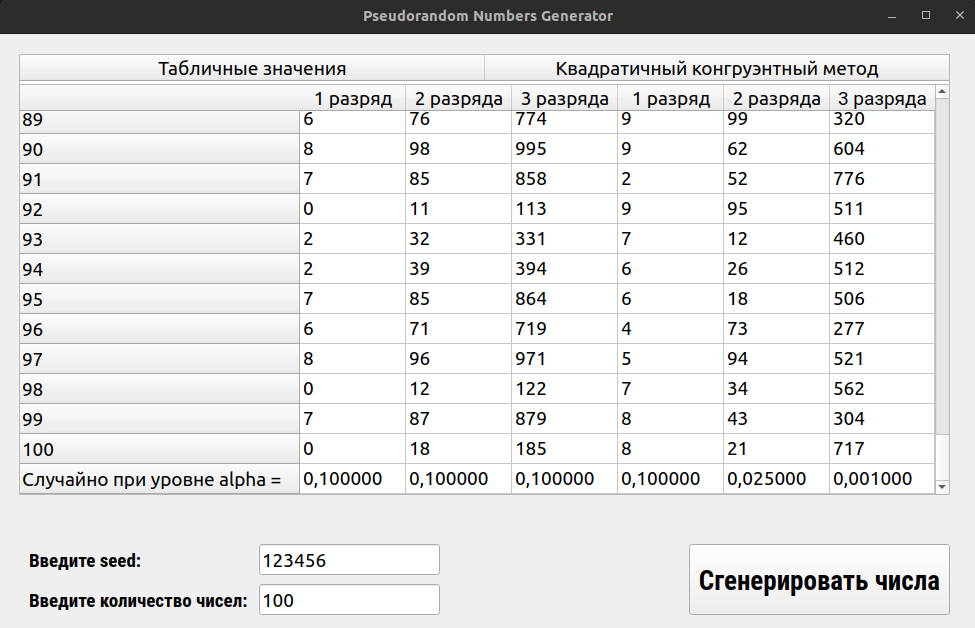
\includegraphics[width=1\linewidth]{images/prng.png}
    \caption{Результат работы программы}
    \label{fig:res}
\end{figure}